\documentclass[conference]{IEEEtran}

\usepackage[utf8]{inputenc}
\usepackage{graphicx}
\usepackage{booktabs}
\usepackage{amsmath}
\usepackage{url}
\usepackage{array}
\usepackage{caption}
\usepackage{hyperref}
\usepackage{listings}
\lstset{
  basicstyle=\ttfamily\footnotesize,
  columns=fullflexible,
  breaklines=true,
  breakatwhitespace=false,
  frame=single,
  xleftmargin=0pt,
  xrightmargin=0pt
}

\begin{document}

% ---------- COVER / TITLE PAGE ----------
\begin{titlepage}
    \centering
    \vspace*{3cm}

    % Big title
    {\Huge \bfseries Online Markov-based Predictive Page Replacement (OM-PPR)\par}

    \vspace{2.5cm}

    % Authors + IDs
    {\large
    Alisha Siddiqui -- 464647\\[0.8em]
    Asawer Ayesha -- 470860\\[0.8em]
    Qura-Tul-Ain Azhar -- 460239\\[1.8em]
    }

    % Department and institution
    {\Large SEECS\\[0.4em]
    NUST\par}

    \vfill
\end{titlepage}

% optional: reset page counter so main paper starts at page 1
\setcounter{page}{1}

% ---------- IEEEtran TITLE / AUTHOR (for header/metadata) ----------
\title{Online Markov-based Predictive Page Replacement (OM-PPR)}

\maketitle

\begin{abstract}
Page replacement policies play a critical role in virtual memory performance by determining which memory pages would be evicted when there is a page fault. Traditional algorithms such as First-In-First-Out (FIFO) and Least Recently Used (LRU) depend on fixed heuristics and do not have the ability to adapt to changing access patterns in modern applications. This paper proposes a solution to this problem called as Online Markov-based Predictive Page Replacement (OM-PPR) algorithm that learns page-to-page transition behaviour at runtime and evicts pages from the frames based on predicted likelihood of a page being reused. The approach ensures lightweight transition statistics and incorporates a safe fallback mechanism to maintain stable performance during cold-start phases. A trace-driven simulation was also conducted to evaluate OM-PPR against FIFO and LRU under locality-dominated, sequential-repeating, and randomized workloads, to support the decision behind the proposal of this algorithm. Experimental results also demonstrate that OM-PPR significantly reduces page faults in locality-rich workloads, achieving up to 42.63\% fault reduction compared to FIFO, with increasing advantages as memory capacity grows. In sequential-repeating workloads, OM-PPR shows progressive improvement, while under randomized access patterns its behavior converges toward classical baselines. These findings suggest that lightweight, online predictive techniques can enhance page replacement decisions in modern operating systems without encountering substantial overhead.
\end{abstract}
\vspace{0.7\baselineskip}

\section{\textbf{Introduction}}

``Virtual memory'' is an important term in modern operating systems, which enables the execution of processes even if the required memory exceeds the system's physical memory \cite{silberschatz2018operating,tanenbaum2015modern}. The memory is partitioned into fixed-size blocks known as ``pages'' and only the required pages are stored in physical memory ``frames''.

Whenever a process attempts to reference a page that is not in main memory, page fault happens \cite{silberschatz2018operating}. Page fault handling involves disk I/O operations, which are several orders of magnitude slower compared with memory access. It is thus essential to reduce the number of page faults in order to optimize performance.

One of the main issues arises when a page fault takes place and all the memory frames are in use. In this scenario, the operating system has no choice but to select a victim page to remove from memory. The efficiency of this process plays a major part in the efficiency of the system \cite{silberschatz2018operating}.
\vspace{0.7\baselineskip}


\section{\textbf{Operating System Background}}

\textbf{Virtual Memory}

Memory management method that provides programs with the illusion of a large memory space that is contiguous.

\textbf{Page}

A block of virtual memory of fixed size.

\textbf{Frame}

A physical area of RAM of a predetermined size.

\textbf{Page Fault}

It occurs when the referred page is not present in the physical memory.

\textbf{Page Replacement Algorithm}

It decides which page needs to be flushed from memory when a page fault occurs and memory is full \cite{silberschatz2018operating,tanenbaum2015modern}.

\section{\textbf{Real-Life Relevance}}

Page replacement needs to be highly effective if the following kinds of environments are to be supported efficiently.

\textbf{Mobile Devices}

Smartphones run on limited RAM memory, with many background applications running. Inefficient page replacement algorithms cause repeated reloading of applications, resulting in battery drain \cite{jiang2005making,levinthal1992performance}.

\textbf{Browsers and Page Replacement Algorithms}

In modern browsers, there can be numerous active tabs, and each consumes memory. Predictive page replacement algorithms can greatly enhance browser experience \cite{lee2017machine,jain2016online}.

\textbf{Cloud Computing and Virtual Machines}

In cloud computing and virtual machines, multiple virtual machines share the same memory. Minimization of page faults means fewer disk I/O operations, and hence efficiency is achieved \cite{megiddo2003arc,corbet2019memory}.
\vspace{0.7\baselineskip}


\section{\textbf{Classical Page Replacement Algorithms}}

\begin{table}[h]
\centering
\caption{Classical Page Replacement Algorithms}
\begin{tabular}{@{}p{1.6cm}p{3.4cm}p{2.4cm}@{}}
\toprule
Algorithm & Principle & Limitation \\ \midrule
FIFO  & Evicts the oldest loaded page & Suffers from Belady's anomaly \\
LRU   & Evicts the least recently used page & High overhead for exact tracking \\
CLOCK & Approximate LRU using reference bits & Reactive, not predictive \\ \bottomrule
\end{tabular}
\end{table}
\vspace{0.7\baselineskip}


All these algorithms rely solely on past access history and do not attempt to predict future accesses \cite{silberschatz2018operating,megiddo2003arc,levinthal1992performance}.

\section{\textbf{Problem Statement}}

The existing algorithms for page replacements are heuristic and not adaptable. They respond to the past and not the future \cite{lee2017machine,jain2016online}. They can potentially incur unnecessary page faults. There is therefore a need for an algorithm that is lightweight and predictive and adapts to memory access patterns and improves the memory management process.

For instance, if a user frequently accesses a web browser tab immediately after viewing an email application, the system can learn this recurring access pattern and assign a higher likelihood to the browser being referenced following the email page \cite{lee2017machine,jain2016online}.

\section{\textbf{Motivation for Proposed Solution}}

In order to overcome these deficiencies, the proposed project shall develop an Online Markov-Based Predictive Page Replacement approach \cite{lee2017machine,jain2016online}. The proposed solution assumes the prediction of the pages that would be accessed in the near future, and the page with the lowest probability would be removed.

\section{\textbf{Proposed Solution and System Design}}

\subsection{Proposed Solution}

\subsubsection{Main Idea}

In this project, we provide an OM PPR (Online Markov Predictive Page Replacement) page replacement strategy.\\
This algorithm's major goal is to predict which page will be used next and prevent that page from being erased from memory.\\
Conventional page replacement techniques, including FIFO and LRU, adhere to set guidelines. When program behaviour shifts, these rules remain unchanged. In order to improve eviction judgments, our algorithm learns page access behaviour throughout execution.
\vspace{0.7\baselineskip}


\subsubsection{Inputs Used by the Algorithm}

When operating, the algorithm makes use of the following data:

\begin{itemize}
\item The reference to the current page
\item The reference to the previous page
\item A transition table that keeps track of page access counts
\item A set of pages that are currently kept in memory frames
\item A history window size of one
\end{itemize}

The technique is kept straightforward and effective by using a short history window.
\vspace{0.7\baselineskip}


\subsubsection{Learning Structure}

The algorithm keeps track of the order in which pages are accessed in a transition table.\\
The definition of the table is:

\textbf{T[a][b] = the number of times page b is accessed following page a.}

As the program runs, this table is updated continuously. It helps in the system's comprehension of typical page access patterns.
\vspace{0.7\baselineskip}


\subsubsection{The Update Rule}

Every time a page is accessed, the count for that page transition is increased by one T if a prior page is present.

T[previous page][current page] = T[previous page][current page] + 1

There is no need for complicated processing because this updating procedure is straightforward.
\vspace{0.7\baselineskip}


\subsubsection{Eviction Decision}

When a page fault occurs and all memory frames are full, the procedure does the following:

\begin{itemize}
\item Calculate the likelihood that each page in memory will be reused.
\item The likelihood is computed using transition counts.
\item Pages without a recorded transition are assigned a probability of zero.
\item The page with the lowest probability is selected for elimination.
\end{itemize}

If no transition data is available for the current page, the technique switches back to LRU or FIFO. This ensures proper behaviour when history is not accessible.
\vspace{0.7\baselineskip}


\subsection{Pseudocode}

\subsubsection{Algorithm 1: Transition Table Update}

Algorithm UpdateTransition(previous page, current page)

\noindent if previous page is not NULL then

\noindent\quad T[previous page][current page] = T[previous page][current page] + 1

\noindent end if

\noindent end Algorithm
\vspace{0.7\baselineskip}


\subsubsection{Algorithm 2: Page Eviction on Page Fault}

Algorithm SelectVictim(current page, Frames)

\noindent if no transition data exists for current page then

\noindent\quad return page selected by LRU or FIFO

\noindent end if

\noindent minimum score = very large value... victim page = NULL

\noindent for each page in Frames do

\noindent\quad if transition exists then

\noindent\qquad score = transition count divided by total transitions

\noindent\quad else

\noindent\qquad score = 0

\noindent\quad end if

\noindent\quad if score is less than minimum score then

\noindent\qquad minimum score = score

\noindent\qquad victim page = current page

\noindent\quad end if

\noindent end for

\noindent return victim page

\noindent end Algorithm
\vspace{0.7\baselineskip}

\subsection{System Architecture}

The system is made up of the following parts:

\begin{itemize}
\item Page reference stream that provides page requests
\item Feature extraction that identifies current and previous pages
\item Predictor that keeps track of the transition table
\item Eviction decision module that chooses a page to remove
\item Memory frames that store active pages
\end{itemize}

The predictor is updated using system feedback following each page reference.

\begin{figure}[h]
\centering
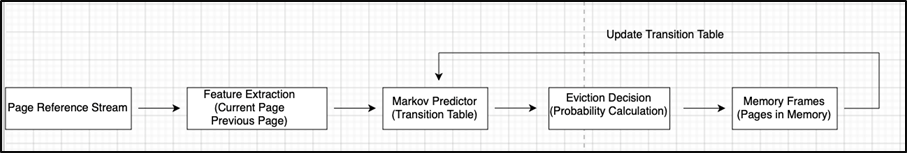
\includegraphics[width=0.9\linewidth]{System architecture.png}
\caption{System Architectural Implementation.}
\end{figure}
\vspace{0.7\baselineskip}


\subsection{Workflow Explanation}

The following is a list of the algorithm's working steps:

\begin{enumerate}
\item Create a blank transition table and memory frames.
\item Read each page reference individually.
\item Count the page as a hit if it is already in memory.
\item In the event of a page fault:
\begin{itemize}
\item If there is free space, load the page.
\item If not, determine the likelihood of reuse and delete the page with the lowest probability.
\end{itemize}
\item Load the updated page into memory.
\item Make changes to the transition table
\item Continue until every page reference has been handled.
\end{enumerate}

Predictive approaches are expected to have these limitations.
\vspace{0.7\baselineskip}


\section{Program Implementation}

A lightweight Python-based simulator was implemented to evaluate FIFO, LRU, and OM-PPR under controlled workloads. OM-PPR maintains online page transition statistics and performs predictive eviction using conditional reuse probabilities, as illustrated in Listings 1 and 2 below.
\vspace{0.7\baselineskip}


\subsection*{Listing 1: OM-PPR eviction decision on page fault}

\begin{lstlisting}
# Evict page with minimum P(page | current); fallback to LRU if cold-start

if current_page in T and sum(T[current_page].values()) > 0:
    victim = min(
        memory,
        key=lambda p: T[current_page].get(p, 0) / sum(T[current_page].values())
    )
else:
    # Cold-start fallback
    victim = min(memory, key=lambda p: last_used.get(p, -1))
\end{lstlisting}
\vspace{0.7\baselineskip}

Listing 1 illustrates the eviction logic used by OM-PPR, where the page with the lowest conditional reuse probability is selected, with a fallback to LRU during cold-start phases.

\subsection*{Listing 2: Online update of page transition statistics}

\begin{lstlisting}
def update_transition(T, prev_page, current_page):
    if prev_page is None:
        return
    T.setdefault(prev_page, {})
    T[prev_page][current_page] = T[prev_page].get(current_page, 0) + 1
\end{lstlisting}
\vspace{0.7\baselineskip}


Listing 2 shows us the implementation where the algorithm learns online which depicts it predictive nature.

\section{Originality and Complexity}

\subsection{Original Contribution}

This solution is unique because:

\begin{itemize}
\item It learns page access behaviour during execution and uses expected reuse to make eviction decisions.
\item Maintaining the algorithm's efficiency and simplicity
\end{itemize}
\vspace{0.7\baselineskip}

\subsection{Complexity Analysis}

\begin{itemize}
\item Space utilisation is dependent on observed page transitions
\item Eviction decisions are based on the number of frames
\item Transition updates take a constant amount of time
\end{itemize}

Due to this, the algorithm is appropriate for evaluation and simulation.
\vspace{0.7\baselineskip}


\section{\textbf{Experimental Results and Case Discussions}}

\subsection{Experimental Setup}

To evaluate the effectiveness of the proposed Online Markov-Based Predictive Page Replacement (OM-PPR) strategy, a trace driven simulation was conducted. This simulator implements a virtual memory system with a fixed number of page frames and processes a sequence of page reference string. It generates a page fault whenever a referenced page is not present in the memory.

The suggested OM-PPR algorithm was compared against two traditional page replacement algorithms: First-in-First-Out (FIFO) and Least Recently Used (LRU). FIFO algorithm has a non-adaptive baseline, while the LRU algorithm works on the recency-based heuristics which is more commonly found in the modern operating systems. Synthetic page reference workloads were designed to imitate different memory access behaviours observed in real applications. These included a locality dominated workload characterized by frequent reuse of a small working set, a sequential workload with periodic repetition, and a randomized workload showing minimal locality. Together, all these workloads also show access patterns seen in real-world interactive application, iterative processing tasks and conflicting scenarios.

The experiments were conducted using multiple memory configurations by changing the number of available page frames. The performance was evaluated using standard operating system metrics, including total page faults, page fault rate and the hit ratio. All the experiments were performed with fixed random seeds to ensure that they are reproducible.
\vspace{0.7\baselineskip}


\subsection{Workloads and Parameters}

The locality-dominated workload was generated by selecting page references from a small set called the ``hot set'' with high probability and from another larger set called the ``cold set'' with low probability. This represented the temporal locality. The sequential workload was created by repeating a fixed cycle of page accesses with small noise to represent the realistic differences across iterations. The randomised workload was generated uniformly over a fixed page range to represent the low-locality behaviour.

Unless stated, each workload contained 2000 total references, and the experiments were repeated across frame sizes 3, 4, 5, and 6.
\vspace{0.7\baselineskip}


\subsection{Metrics}

The following metrics were used for evaluation of the different page replacement algorithms:

\begin{enumerate}
\item Total Page Faults: These were the number of references that required a page to be loaded in the memory (i.e., the page was not present in the memory).
\item Page Fault Rate: Total Page Faults / Total Page References.
\item Hit Ratio: Pages already present in the memory / Total Page References
\end{enumerate}

These metrics directly reflected the effectiveness of the replacement decision in minimising costly page faults.
\vspace{0.7\baselineskip}


\subsection{Experimental Results}

After implementing this strategy in a program, the results below were observed.

\begin{table*}[t]
\centering
\caption{Comparison of Page Faults for FIFO, LRU, OM-PPR Across Different Workloads.}
\resizebox{\textwidth}{!}{%
\begin{tabular}{@{}lllllllll@{}}
\toprule
\textbf{Workload} & \textbf{Frames} & \textbf{Reference String} &
\textbf{FIFO Faults} & \textbf{LRU Faults} & \textbf{OM-PPR Faults} &
\textbf{OM-PPR HitRatio} & \textbf{Faults per 1000} & \textbf{Imp vs FIFO \%} \\
\midrule
Locality & 3 & 2000 & 1127 & 1111 & 1053 & 0.4735 & 526.5 & 6.57 \\
Locality & 4 & 2000 & 887  & 830  & 716  & 0.642  & 358   & 19.28 \\
Locality & 5 & 2000 & 706  & 591  & 439  & 0.7805 & 219.5 & 37.82 \\
Locality & 6 & 2000 & 577  & 412  & 331  & 0.8345 & 165.5 & 42.63 \\
Sequential-Repeat & 3 & 2000 & 1974 & 1975 & 1972 & 0.014  & 986   & 0.1 \\
Sequential-Repeat & 4 & 2000 & 1974 & 1973 & 1876 & 0.062  & 938   & 4.96 \\
Sequential-Repeat & 5 & 2000 & 1973 & 1964 & 1675 & 0.1625 & 837.5 & 15.1 \\
Sequential-Repeat & 6 & 2000 & 1967 & 1951 & 1356 & 0.322  & 678   & 31.06 \\
Random & 3 & 2000 & 1807 & 1807 & 1809 & 0.0955 & 904.5 & -0.11 \\
Random & 4 & 2000 & 1736 & 1733 & 1749 & 0.1255 & 874.5 & -0.75 \\
Random & 5 & 2000 & 1669 & 1670 & 1681 & 0.1595 & 840.5 & -0.72 \\
Random & 6 & 2000 & 1581 & 1591 & 1610 & 0.195  & 805   & -1.83 \\
\bottomrule
\end{tabular}%
}
\end{table*}
\vspace{0.7\baselineskip}


Table II summarises the total page faults observed for FIFO, LRU, and the suggested Online Markov-Based Predictive Page Replacement Algorithm (OM-PPR) strategy across different workloads and memory configurations. The results that we receive are for locality-dominated, sequential repeating, and randomised access with varying numbers of page frames.

\subsubsection*{a) Locality dominated Workload}

\begin{figure}[h]
\centering
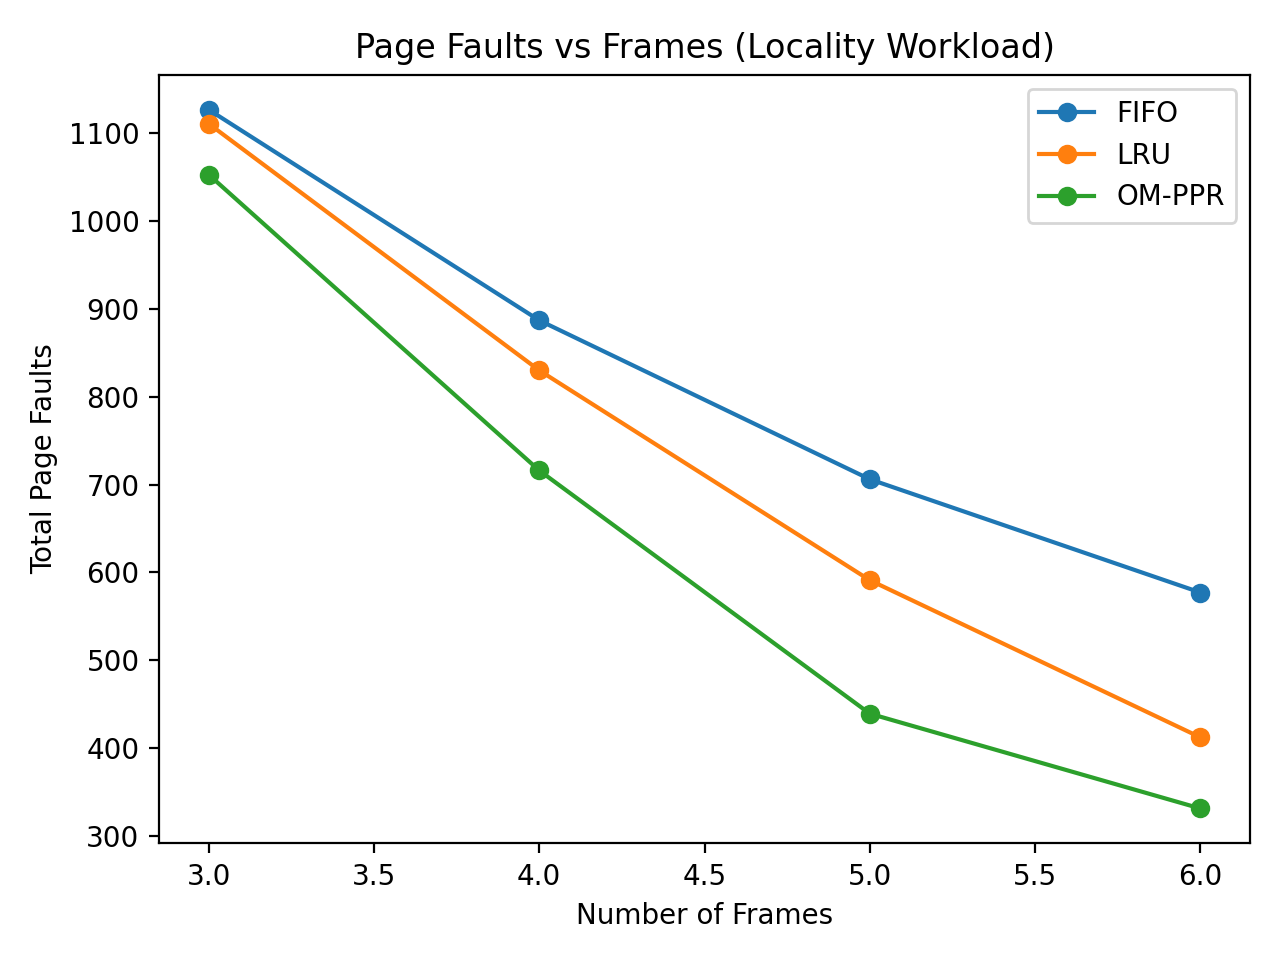
\includegraphics[width=0.7\linewidth]{faults_vs_frames_Locality.png}
\caption{Locality Workload - Page Faults Vs Frames (FIFO, LRU, OM-PPR)}
\end{figure}
\vspace{0.7\baselineskip}


In locality dominated workloads, it is observed that OM-PPR consistently performed better than FIFO and LRU across all frame sizes. With three frames, OM-PPR had a 6.57\% reduced page fault rate as compared to FIFO. As the number of frames increased, the advantage of OM-PPR became more prominent, showing a 42.63\% reduction in the page faults at six frames. Similarly, the hit ration increased from 47.53\% to 83.45\% which showed the effectiveness of the core idea of OM-PPR algorithm, i.e., learning repeated transition patterns under strong temporal locality.

\subsubsection*{b) Sequential Repeating Workload}

\begin{figure}[h]
\centering
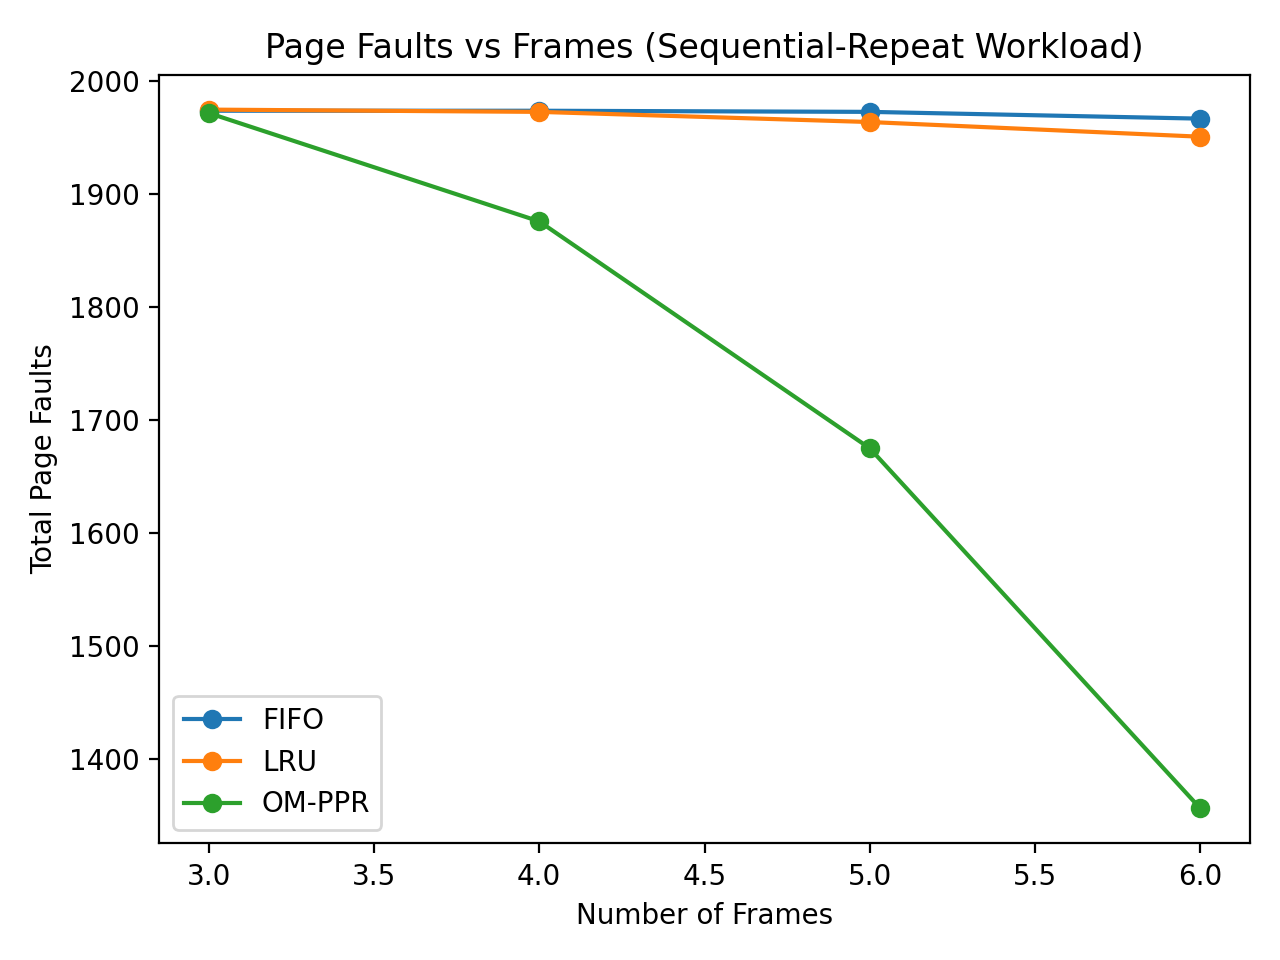
\includegraphics[width=0.7\linewidth]{faults_vs_frames_Sequential-Repeat.png}
\caption{Sequential-Repeat Workload - Page Faults vs Frames (FIFO, LRU, OM-PPR)}
\end{figure}
\vspace{0.7\baselineskip}


For the sequential repeating workload, OM-PPR showed a gradual improvement as the number of frames increased. Although for lower page frames, such as three, the performance gain did not appear to be too much (only 0.1\%, see Table II), the algorithm achieved a 31.06\% reduction in the page faults as compared to FIFO at six frames. This behaviour suggests that the algorithm's ability to learn patterns in the sequences over time, particularly once enough frames were provided, allows for a stable pattern retention.

\subsubsection*{c) Random Workload}

\begin{figure}[h]
\centering
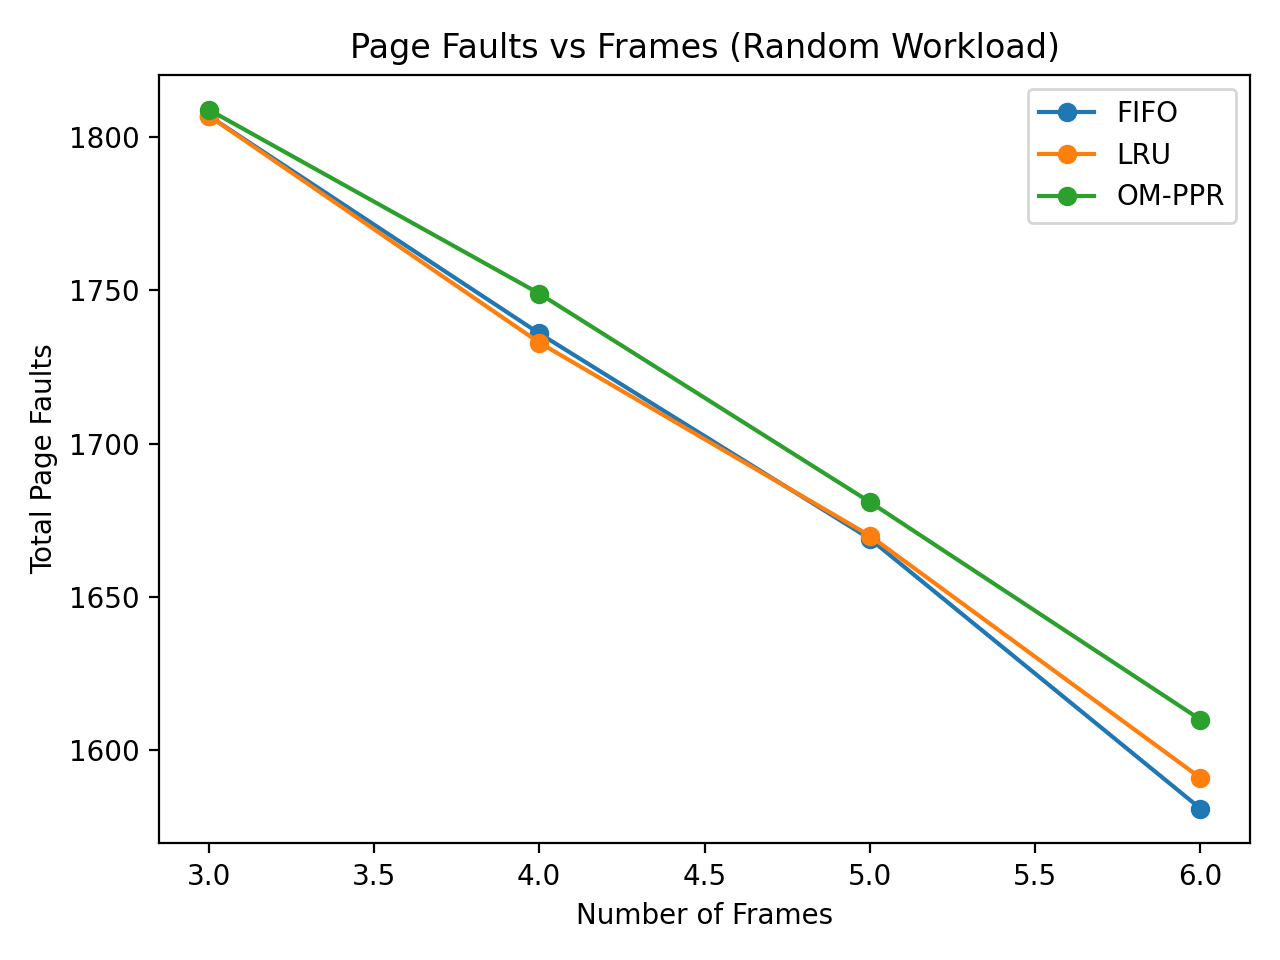
\includegraphics[width=0.7\linewidth]{faults_vs_frames_Random.png}
\caption{Random Workload - Page Faults vs Frames (FIFO, LRU, OM-PPR)}
\end{figure}
\vspace{0.7\baselineskip}

Under randomised workloads, OM-PPR exhibited similar page fault behaviour as compared to FIFO and LRU. In fact, in some cases, OM-PPR displayed slightly higher number of page faults (up to 1.83\% worse than FIFO). This outcome is expected as random-access patterns provide limited reference for a transition-based prediction.
\vspace{0.7\baselineskip}


\section{\textbf{Discussion}}

The experimental results discussed in Section 6.4 highlight the strengths and limitations of our proposed page replacement algorithm, Online Markov Predictive Page Replacement (OM-PPR) in relation to access pattern characteristics. In workload where there is strong locality, the algorithm performed significantly better than the traditional algorithms. It reduced the page faults by clearly observing a page-to-page transition behaviour, thus, allowing it to retain pages with a higher predicted use probability. This predictive capability of the algorithm allows it to outperform the traditional heuristic based approaches such as FIFO and LRU. Figure 1 clearly shows this comparison.

According to the results in Table II and the graph in figure 2, in sequential-repeating workloads, performance gains increased significantly with the increase in the size of memory available in terms of page frames. This suggests that OM-PPR gains benefit from a greater number of frames to preserve learned transition histories across iterations, allowing the predictive nature of the algorithm to stabilise. The relatively small improvement at low frame counts can be accounted to frequent evictions of pages from the frames leading to disruptions in learned patterns.

On the other hand, in randomised workloads, the absence of consistent access structure reduces the prediction capability of the algorithm. In such cases, OM-PPR as seen by Table II and Figure 3, the algorithm converges towards baseline behaviour, sometimes incurring minor overhead due to mispredictions. However, this result can also be used to provide this context, that the algorithm OM-PPR does not overfit or exploit unrealistic assumptions.

Overall, these results indicate that OM-PPR is the most effective in real-world situations where temporal locality and phased execution is present. These two characteristics are commonly found in real world, interactive applications, iterative programs and multi-programmed operating systems.
\vspace{0.7\baselineskip}


\section{\textbf{Limitations and Future Works}}

While the proposed Online Markov-based Predictive Page Replacement (OM-PPR) algorithm shows significant performance improvements under locality-rich and repetitive workloads, there are several limitations which are observed as well.

Firstly, OM-PPR displays a cold-start phase, during which there is insufficient transition history which limits the prediction accuracy. Although there is a Least Recently Used (LRU) fallback mechanism ensuring a stable behaviour during this phase, early execution performance still resembles traditional heuristic results.

Secondly, the algorithm maintains transition statistics or count to model a page-to-page behaviour for its predictive mechanism which introduces an additional memory overhead compared to FIFO and LRU. In large address spaces, the overhead might require bounded data structures, aging, or decay mechanisms to remain practical and affordable.

Thirdly, OM-PPR provides a very limited benefit under highly randomised access patterns, as observed in the Section 6.4 of experimental results. The prediction accuracy decreases due to the absence of a structured pattern. In such cases, the performance becomes similar to the baseline algorithms and might even incur minor misprediction overhead.

Future work can include incorporating decay-based learning to adapt to more rapidly changing phases, which can include exploring hybrid designs that combine OM-PPR with recency or frequency-based heuristics and evaluating the approach using real application traces from browsers, databases, or virtualised environment to further extend its practical applicability.
\vspace{0.7\baselineskip}


\section{\textbf{Conclusion}}

This research paper successfully evaluated an Online Markov-based Predictive Page Replacement algorithm designed to improve the virtual memory management by learning the page transition pattern at runtime. Unlike traditional heuristic-based replacement policies, OM-PPR clearly estimates the future page reuse likelihood and adapts its eviction decisions according to it.

The simulation, in Section 6, allowed us to demonstrate that OM-PPR significantly reduces page faults in locality-dominated workloads, achieving up to 42.63\% page fault reduction compared to FIFO, and provides increasing benefits in sequential-repeating workloads as the memory capacity grows. Under the randomised-access patterns, OM-PPR depicted a baseline behaviour which allowed us to analyse the limitations of these predictive approaches.

By combining the lightweight online learning with a safe fallback mechanism, OM-PPR offers us a practical and adaptable enhancement to traditional page replacement algorithms. The results suggest that predictive, learning-based techniques can play an important role in modern operating systems executing wide range and rapidly changing workloads.

\vspace{0.7\baselineskip}

\begin{thebibliography}{14}

\bibitem{silberschatz2018operating}
A.~Silberschatz, P.~B. Galvin, and G.~Gagne,
\emph{Operating System Concepts}, 10th ed.
New York, NY, USA: Wiley, 2018.

\bibitem{tanenbaum2015modern}
A.~S. Tanenbaum and H.~Bos,
\emph{Modern Operating Systems}, 4th ed.
Boston, MA, USA: Pearson, 2015.

\bibitem{megiddo2003arc}
N.~Megiddo and D.~S. Modha,
``ARC: A Self-Tuning, Low Overhead Replacement Cache,''
\emph{Proceedings of the 2nd USENIX Conference on File and Storage Technologies (FAST)}, 2003.

\bibitem{jiang2005making}
S.~Jiang and X.~Zhang,
``Making LRU Friendly to Weak Locality Workloads: A Novel Replacement Algorithm,''
\emph{IEEE Transactions on Computers}, vol. 54, no. 8, pp. 939--952, Aug. 2005.

\bibitem{lee2017machine}
M.~E. Lee, K.~H. Kim, and Y.~S. Kim,
``Machine Learning Based Cache Replacement Policy,''
\emph{International Journal of Computer Science and Network Security}, vol. 17, no. 3, pp. 1--7, 2017.

\bibitem{jain2016online}
A.~Jain and C.~Lin,
``Online Learning Algorithms for Predictive Caching,''
\emph{Proceedings of the IEEE International Conference on Big Data}, 2016.

\bibitem{corbet2019memory}
J.~Corbet,
``Memory Management in the Linux Kernel,''
\emph{Linux Weekly News (LWN)}, 2019.

\bibitem{levinthal1992performance}
D.~Levinthal,
``Performance Analysis of Page Replacement Algorithms,''
\emph{ACM Computing Surveys}, vol. 24, no. 1, pp. 1--42, 1992.

\bibitem{smith1982cache}
A.~J. Smith, Cache memories, ACM Computing Surveys, 1982.

\bibitem{podlipnig2003survey}
S.~Podlipnig and L.~Böszörmenyi, Survey of web cache replacement strategies, ACM Computing Surveys, 2003.

\bibitem{chou1985evaluation}
A.~Chou and J.~DeWitt, Evaluation of buffer management strategies, VLDB, 1985.

\bibitem{zhou2001multi}
Y.~Zhou, J.~Philbin, and K.~Li, Multi queue replacement algorithm, USENIX, 2001.

\bibitem{squillante1993processor}
M.~S. Squillante and E.~D. Lazowska, Processor cache affinity information, IEEE TPDS, 1993.

\bibitem{pattersonhennessy}
D.~A. Patterson and J.~L. Hennessy, Computer Organization and Design, Morgan Kaufmann.

\end{thebibliography}

\end{document}
